\documentclass[blue, normal]{./templete/qyxfnote}

\usepackage{xeCJK}
\usepackage{multicol}
\usepackage{amsmath}
\usepackage{amssymb}
\usepackage{graphicx}
\usepackage{subcaption}
\usepackage{draftwatermark}
\SetWatermarkText{钱院学辅}
\SetWatermarkLightness{0.9}
\SetWatermarkScale{0.9}

\title{大物答案}
\author{钱院学辅大物编写小组}
\date{\today}


\newcommand{\di}[1]{\mathrm{d}#1}
\newcommand{\p}[2]{\frac{\partial #1}{\partial #2}}
\newcommand{\pp}[2]{\frac{\partial ^2 #1}{\partial #2 ^2}}
\newcommand{\dy}[2]{\frac{\di{#1}}{\di{#2}}}
\newcommand{\ddy}[2]{\frac{\mathrm{d} ^2 #1}{\mathrm{d} #2 ^2}}
\newcommand{\zbj}[4]
{
	\draw (0,0) node[below left] {$ O $};
	\draw [->] (#1,0) -- (#2,0) node[right] {$ x $};
	\draw [->] (0,#3) -- (0,#4) node[right] {$ y $};
}


\begin{document}
	\maketitle
	\newpage
	\versiontext{\today}
	\newpage
	\updatetext{此版本为试用版}
	\tableofcontents
	\newpage
	\begin{multicols}{2}

	\section{第一章}
	\subsection{选择题}
		1.A\\
		\indent
		如图1.1,对M,在x方向上:
		\vspace{-1em}
		\begin{figure}[htbp]
			\centering
			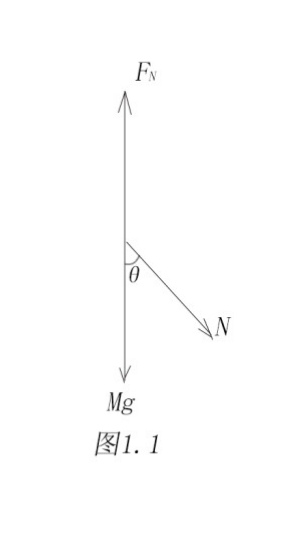
\includegraphics[width=10em,height=15em]{Chp1_illus1.png}
			\quad
			\centering
			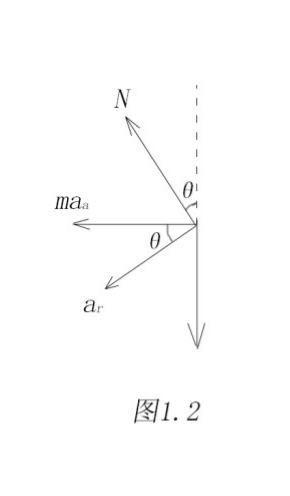
\includegraphics[width=10em,height=15em]{Chp1_illus2.png}
		\end{figure}
		\vspace{-3.5em}
		\begin{gather}
		N\cos\theta=Ma_a\text{(M对地)}\\
		\text{如图1.2,对m,以M为参考系,m受一惯性}\notag\\
		\text{力,合加速度沿二者接触面。沿x,y方向分解:}\notag\\
		mg-N\cos\theta=ma_r\sin\theta\\
		ma_a+N\sin\theta=ma_r\cos\theta\\
		\text{(1)代入(2),(2)(3)联立解得:}\notag\\
		a_r=\dfrac{(M+m)g\sin\theta}{M+m{\sin\theta}^2}\notag
		\end{gather}
		2.B\\ \indent
		如图1.3,$u=v\cos\theta$,v不变而$\theta$增大,需要u减小。\\
		\vspace{-3.5em}
		\begin{figure}[htbp]
			\centering
			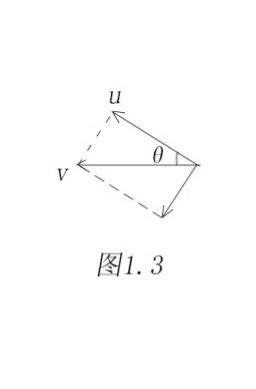
\includegraphics[width=6.5em,height=10em]{Chp1_illus3.png}
			%\caption{}
			\label{fig:Chp1_illus2}
		\end{figure}
		\vspace{-4.5em} \\
		3.A\par
		匀速圆周运动的速度、加速度(受力)均是大小不变、方向时刻变化。
		注意一个矢量为常量包括大小和方向两个方面。否则就是变化的量。\\
		4.B\par
		以前面的货车为参考系,货车静止,火车速率为$v_1-v_2$,加速度为$a$(反向),那么火车最多前进$s=\dfrac{{(v_1-v_2)}^2}{2a}$。要求$d>s$,故选B。或采用地面参考系的追逐问题法,计算从$v_1\text{减速到}v_2$两车走过的距离之差:$s=\dfrac{{v_1}^2-{v_2}^2}{2a}-v_2\cdot \dfrac{v_1-v_2}{a}=\dfrac{{(v_1-v_2)}^2}{2a}$\\
		5.C\par
		两次求导得:$a=30t\neq$常数而大于零。\\
		6.B\par
		求导得:$v=8t-6t^2,a=8-12t$\par
		$\text{令}y=0\Rightarrow t=0\text{(舍去)或}2$,代入得结果。\\
		7.B\par
		物体做匀加速直线运动。\vspace{-1em}
		\begin{gather*}
		s=\dfrac{b}{\cos\alpha},a=g\sin\alpha\\
		t=\sqrt{\dfrac{2s}{a}}=\sqrt{\dfrac{4b}{g\sin(2\alpha)}}
		\end{gather*}
		\par $t$最小时,$\sin(2\alpha)$最大,$\alpha=45^\circ$。\\
		8.B\par 
		类比从静止出发的匀加速直线运动。$t=\dfrac{2\cdot 2\pi}{\beta}$\\
		9.B\par 
		曲线的定义:“动点运动方向连续变化的轨迹”\footnote{来源:汉典网http://www.zdic.net/c/2/111/299079.htm}。A,C的反例:匀速圆周运动。\\
		10.D\par 
		反例:平抛运动\\		
		\subsection{填空题}
		11.\ 0\qquad2g\\
		\indent
		设A、B质量为m。抽走C之前,弹簧中的弹力大小为mg。撤去C时,弹簧长度未突变,弹力不变,A受合力为0;支持力则消失。\par
		故$a_A=0;a_B=\dfrac{mg+mg}{m}=2g$,竖直向下。\\
		12.\ $\dfrac{25}{12}\pi\ rad/s^2$ \qquad$\dfrac{24}{5}s$
		\begin{gather*}
		\text{简单公式应用。}\theta=60\times2\pi=120\pi\\
		\beta=\dfrac{\omega_2^2-\omega_1^2}{2\theta}=\dfrac{25}{12}\pi\ rad/s^2\\
		\delta t=\dfrac{\omega_2-\omega_1}{\beta}=\dfrac{24}{5}s
		\end{gather*}
		13. $m(\sin\theta-\omega^2l\sin\theta\cos\theta)$
		\vspace{-1em}
		\begin{figure}[htbp]
			\centering
			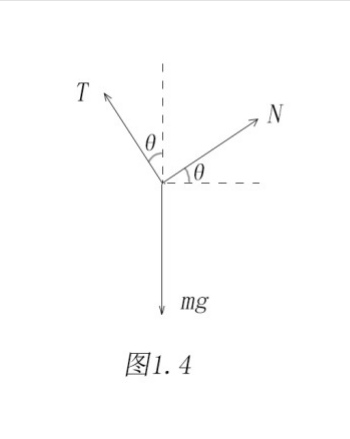
\includegraphics[width=15em, height=15em]{Chp1_illus4.png}
			%\caption{}
			\label{fig:c1}
		\end{figure}
		\vspace{-3em}
		\begin{gather*}
		\text{如图1.4,在x,y方向上分解受力,得:}\\		
		T\sin\theta-N\cos\theta=m\omega^2l\sin\theta\\
		T\cos\theta+N\sin\theta=mg\\
		\text{联立可解得T、N的大小。}
		\end{gather*}
		14.\ $2\sqrt{\dfrac{r}{g}}$ \qquad $2\sqrt{\dfrac{r}{g}}$
		\vspace{-0.5em}
		\begin{gather*}
		\text{设弦与PC的夹角为}\theta,\text{则有}\\
		s=2r\cos\theta,a=g\cos\theta\\
		t=\sqrt{\dfrac{2s}{a}}=2\sqrt{\dfrac{r}{g}}
		\end{gather*}
		15.\ $4\sqrt{5}m/s$ \qquad $16m/s^2 $ 
		\vspace{-1em}
		\begin{gather*}	
		\text{抛物线的切线方向即为质点的速度方向,且}x=4t\\
		\therefore \dfrac{v_y}{v_x}=\dy{y}{x}=x\Rightarrow v_y=4x=16t\\
		\therefore t=2\text{时,}v_y=8\mathrm{m/s},
		v=\sqrt{{v_x}^2+{v_y}^2}=4\sqrt{5}\mathrm{m/s}\\
		v_x\text{不变,}a=a_y=\dy{v_y}{t}=16\mathrm{m/s^2}
		\end{gather*}
		16. 长度、质量、时间\par
		见课本,解答略。\\
		17. 3\quad 3\quad 6\par
		x分别对t求一阶两阶导即是v、a,由图像即可判断其正负号。\\
		18. $y={(x+5)}^3$
		\vspace{-1em}
		\begin{gather*}\text{由题,}x=2t-5\Rightarrow 2t=x+5\\
		\text{代入}y=8t^3={(2t)}^3\text{,消去t即可}
		\end{gather*}	
		19. $\dfrac{1}{2}g$\qquad 竖直向下\par
		初始时受力平衡,两根弹簧上力均为$\dfrac{1}{2}mg$;一根断掉后,向上的力减半,则小球受的合力是$\dfrac{1}{2}mg$,竖直向下。\\
		20.\ 9m/s 
		\vspace{-1em}
		\begin{gather*}\text{(SI)} x=3t+6t^2-2t^3\xrightarrow{\text{求导}}v=3+12t-6t^2\\
		\xrightarrow{\text{求导}}a=12-12t\\\
		令a=0\ \text{解得}\ t=1\xrightarrow{\text{代入得}} v(1)=9\mathrm{m/s}
		\end{gather*}
		\subsection{计算题}
		%21,22,24题对原作者代码有改动
		21.
		\begin{gather*}
		\text{由图知:}\\
		\tan\alpha=\dfrac{|\vec{a}_n|}{|\vec{a}_\tau|}=\dfrac{\dfrac{v^2}{R}}{\dy{v}{t}}\\
		\therefore \dy{v}{t}\frac{1}{v^2}=\frac{1}{R\tan\alpha}\\
		\text{积分得:}-\frac{1}{v}=\frac{1}{R\tan\alpha}t+C\\
		\text{代入}t=0,v=v_0\\
		\therefore \frac{1}{v_0}-\frac{1}{v}=\frac{1}{R\tan\alpha}t
		\ \text{即}v=\frac{v_0R\tan\alpha}{\tan\alpha-v_0t}
		\end{gather*}
		22.
		\begin{gather*}
		\vec{v}=\dy{s}{t}\vec{\tau}=(c+2dt)\vec{\tau}\\  
		\vec{a}_n=\frac{v^2}{R}\vec{n}=\frac{(c+2dt)^2}{R}\vec{n}\\
		\vec{a}_\tau=\dy{v}{t}\vec{\tau}=2d\vec{\tau}\\
		\text{令}|\vec{a}_n|=|\vec{a}_\tau|,
		\text{则}\frac{(c+2dt)^2}{R}=2d\\
		\therefore t_1=\frac{\sqrt{2dR}-c}{2d}\left(t_2=\frac{-\sqrt{2dR}-c}{2d}<0\text{,舍去}\right)\\
		\therefore\text{要使t}\geqslant\text{0,条件为}\sqrt{2dR}-c\geqslant0,\text{即}2dR\leqslant c^2
		\end{gather*}
		23.
		\begin{gather*}
		-kx=a=\dy{v}{t}=\dy{v}{x}\cdot \dy{x}{t}=\dy{v}{x}\cdot v\\
		\text{分离变量,积分得:}-\dfrac{1}{2}kx^2=\dfrac{1}{2}v^2+C_1\\
		\text{令}C=2C_1,\text{则}-kx^2=v^2+C\\
		\text{代入}x=x_0,v=v_0\text{\,得:}C=-(kx_0^2+v_0^2)\\
		\text{整理得:}v=\pm\sqrt{kx_0^2+v_0^2-kx^2}
		\end{gather*}
		24.
		\begin{align*}
		(1)v&=10\left(1-\frac{t}{5}\right)\\
		&=-2t+10\\
		\dy{x}{t}&=-2t+10
		\end{align*}
		\vspace{-2.5em}
		\begin{gather*}
		\text{积分得:}x=-t^2+10t+c\\
		\text{代入}t=0,x=0,\quad \therefore x=-t^2+10t\\
		\text{代入}t=10s\\
		\therefore x=0.\quad
		\therefore\text{坐标为}0\\
		(2)\text{令}x=10m,\therefore t^2-10t+10=0\\
		\therefore t=5\pm\sqrt{15}s\\
		\text{令}x=-10m,\therefore t^2-10t+10=0\\
		\therefore t=5+\sqrt{35}(5-\sqrt{35}<0,\text{舍去})\\
		\therefore\text{时刻为}5-\sqrt{15}\ s,5+\sqrt{15}\ s\text{或}5+\sqrt{35}\,s\\
		(3)\text{令}v=0,\therefore t=\ 5s\\
		\therefore t\in[0,5],\quad s=x=-t^2+10t\\
		t\in[5,+\infty),\quad s=s(5)+[s(5)-x]=25\\+[25-(-t^2+10t)]
		=t^2-10t+50\\
		\therefore s=
		\begin{cases}
		-t^2+10t,&t\in[0,5)\\
		t^2-10t+50,&t\in[5,+\infty)
		\end{cases}
		\end{gather*}
	

	
	\section{第二章}
	

	\subsection{选择题}
	\noindent
	1.C\par
	质点沿力方向位移为零。$\therefore A=0$.\\
	2.B\par
	$B$离开$A$时为弹簧恢复原长的时刻(该时刻之后,$A$受到弹簧拉力,加速度为负,$v_A<v_B$.)\par
	此时$v_A=v_B$.由动能定理:
	\begin{align*}
	\frac{1}{2}mv_A^2+\frac{1}{2}mv_B^2-0=\frac{1}{2}kd^2\\
	\therefore{}E_B=\frac{1}{2}mv_B^2=\frac{1}{4}kd^2
	\end{align*}
	3.C\par
	对$\vec{r}$求导:
	\begin{align*}
	\vec{v}&=\frac{\di{\vec{r}}}{\di{t}}\\
	&=-\frac{2\pi}{T}A\sin\frac{2\pi t}{T}\vec{i}+\frac{2\pi}{T}B\cos\frac{2\pi t}{T}\vec{j}
	\end{align*}
	\par$t=0$时,
	\begin{align*}
	v_1&=\sqrt{v_{x1}^2+v_{y1}^2}\\
	&=\sqrt{0^2+\left(\frac{2\pi}{T}B\right)^2}=\frac{2\pi}{T}B
	\end{align*}
	\[\therefore{}E_{k1}=\frac{1}{2}mv_1^2=\frac{2m\pi^2}{T^2}\left(B^2\right)\\\]
	\par$t=\frac{T}{4}$时,
	\begin{align*}
	v_2&=\sqrt{v_{x2}^2+v_{y2}^2}\\
	&=\sqrt{\left(-\frac{2\pi}{T}A\right)^2+0^2}=\frac{2\pi}{T}A
	\end{align*}
	\begin{gather*}
	\therefore{}E_{k2}=\frac{1}{2}mv_2^2=\frac{2m\pi^2}{T^2}\left(A^2\right)\\
	\therefore\Delta{}E_k=\frac{2\pi^2}{T^2}(B^2-A^2)
	\end{gather*}
	4.D\par
	由动量定理:
	\[0=m_1v_1-m_2v_2\]
	\[\therefore{}v_2=\frac{m_1}{m_2}v_1\]\par
	由机械能守恒:
	\begin{align*}
	E_p &=\frac{1}{2}m_1v_1^2+\frac{1}{2}m_2v_2^2\\
	&=\frac{m_1v_1^2+\frac{m_1^2v_1^2}{m_2}}{2}\\
	&=\frac{m_1v_1^2\left(m_1+m_2\right)}{2m_2}
	\end{align*}
	5.B\par
	(2):既然小车能在水平面上停止,说明水平面是粗糙的,有摩擦力做功。因此不满足机械能守恒。\par
	(4):重力做正功,摩擦力做负功,符号相反。\\
	6.D\par
	弹簧上任意一点弹力相同,记为N。截去一半后,伸长量缩短了一半,而弹力不变,因此k变为原来的两倍。\par
	并联在一起后,每一根弹簧受力为原先的一半。由$F=kA$,伸长量为原来的$\frac{1}{4}$。\par
	写成数学式子如下:
	\begin{align*}
	E_k &=2\times\left(\frac{1}{2}k'A'^2\right)\\
	&=\left(2k\right)\times\left(\frac{1}{4}A\right)^2\\
	&=\frac{1}{8}kA^2
	\end{align*}
	7.D\par 
	物体沿重力方向的位移为负,因此重力做负功。其它选项,物体沿推力方向有位移,因此推力做功,A错误;推力功与摩擦力做的功和重力做的功之和等值反号,因此BC错误。\\
	8.C\par 
	若合外力的冲量为0,则由冲量定义$\vec{I}=\int_{t1}^{t2}\vec{F}\di{t}$知,$\vec{F}=\vec{0}$,因此合外力做的功为0。其它选项,AD可举匀速圆周运动的反例;对于B,合外力不为0,必有加速度,而质量不改变,因此$\vec{v}$必然改变,即动量必改变。\\
	9.B\par 
	由动能表达式$E_k=\frac{p^2}{2m}$,在动量相同的情况下,质量越大,动能越小,因此选B\\
	10.A\par 
	设小球重力为$G$,弹簧弹性系数为$k$,则$G=kd$,再设最低点时弹簧伸长$h$。以弹簧原长的高度为基准,释放前和最低点为始末态,应用机械能守恒:
	\[Gh=\frac{1}{2}kh^2\]
	解得$h=2d$
	
	\subsection{填空题}
	
	11.$31J$
	\[A=\int_{0.5}^{1}F\di{x}=\int_{0.5}^{1}(52.8x+38.4x^2)\di{x}=31(J)\]
	12.$24J$ $4m/s$\par 
	\[A=\int_{1}^{4}F\di{x}=\int_{1}^{4}(3+2x)\di{x}=24(J)\]
	\[\text{由动能定理:}\frac{1}{2}mv^2=24,\quad \therefore v=4(m/s)\]
	13.$\frac{GMm}{6R}$ \qquad $-\frac{GMm}{3R}$
	\begin{gather*}
	\text{卫星运动的向心力由万有引力提供,}\therefore m\frac{v^2}{3R}=G\frac{Mm}{(3R)^2}\\
	\therefore E_k=\frac{1}{2}mv^2=\frac{GMm}{6R}\\
	\text{由引力势能公式:}E_p=-\frac{GMm}{r}=-\frac{GMm}{3R}
	\end{gather*}
	14.1296
	\begin{gather*}
	\text{由牛顿第二定律:}F=ma,\qquad t^2=2a=2\ddy{x}{t},\\
	\text{再由初始条件}t=0,x=0\text{且}v=0, \text{解得}x=\frac{1}{24}t^4\\
	\text{由此可知}x=54m\text{时}, t=6s\\
	A=\int_{0}^{6}F\di{x}=\int_{0}^{6}t^2\di{(\frac{1}{24}t^4)}\\
	\therefore A=1296J
	\end{gather*}
	15.$19.8m/s$\par
	(小行星的物理量下标为1)
	\begin{gather}
	\text{向心力由万有引力提供,}\therefore m\frac{v_1^2}{R_1}=G\frac{Mm}{R_1^2}\notag\\
	\text{将}M=\frac{4}{3}\pi R^3\rho\text{代入,得}v_1=\sqrt{G\frac{4}{3}\pi\rho R_1^2}\\
	\text{由地球上重力为}g=9.8m/s,mg=G\frac{Mm}{R_2^2}\notag\\
	\therefore g=G\frac{4}{3}\pi R_2\rho.\text{则}G\frac{4}{3}\pi\rho=\frac{g}{R_2}\notag\\
	\text{代入(1),}v_1=\sqrt{\frac{gR_1^2}{R_2}}\approx19.8(m/s)\notag
	\end{gather}
	16.$\sqrt{\frac{2Mgh}{m+M}}$ \qquad $\frac{m^2gh}{M+m}$
	\begin{gather}
	\text{由动量定理:}mv_1=Mv_2\\
	\text{由机械能守恒:}mgh=\frac{1}{2}mv_1^2+\frac{1}{2}Mv_2^2\\
	\text{联立(1)(2)解得:}v_1=\sqrt{\frac{2Mgh}{m+M}}\notag\\
	v_2=\sqrt{\frac{2m^2gh}{(m+M)M}}\notag\\
	\text{由动能定理知,物块对滑道做的功就是滑道动能改变量}\notag\\
	\text{即}\frac{1}{2}Mv_2^2=\frac{m^2gh}{M+m}\notag
	\end{gather}
	17.第i个质点所受合力做的功(类似说法均正确)\\
	18.1m/s \qquad 200J\par
	船员用200N的力拉绳子,由牛顿第三定律,绳子也给船员(和船)200N的拉力。以人和船为对象应用牛顿第二定律,解得:
	\[a=\frac{F}{m}=0.5m/s^2\]
	因此第2秒末速率为1m/s,增加的动能就是
	\[E_k=\frac{1}{2}mv^2=\frac{1}{2}\times400\times1^2=200(J)\]
	19.$\left(\frac{1}{r_2}-\frac{1}{r_1}\right)GMm$ 
	\begin{gather*}
	\text{由机械能守恒,}0+E_{p1}=E_k+E_{p2}\\
	\therefore E_k=E_{p2}-E_{p1}=\left(\frac{1}{r_2}-\frac{1}{r_1}\right)\\
	\text{以两个质点为系统,仅有万有引力(内力)做功,因此由质点系动能定理:}\\
	A=E_k=\left(\frac{1}{r_2}-\frac{1}{r_1}\right)GMm
	\end{gather*}
	20.$0.8\sqrt{2}$\par
	\centering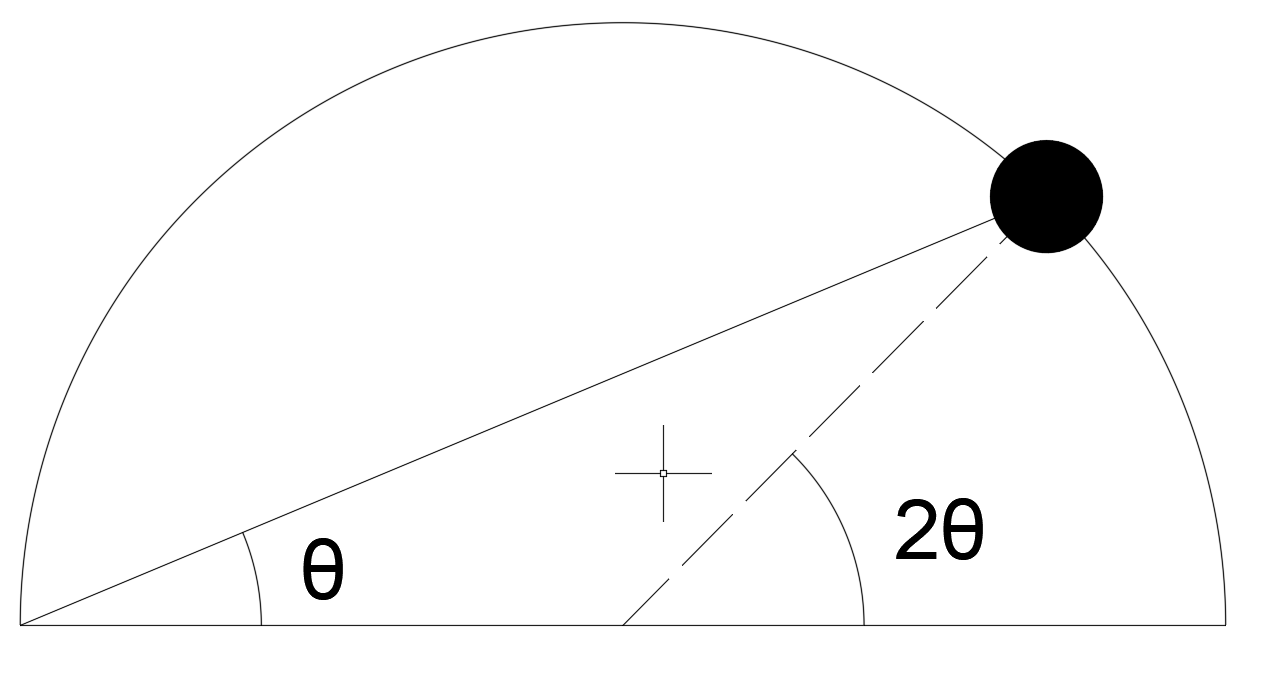
\includegraphics[height=100pt]{Chp2_illus1.png}\\
	图1
	\begin{align*}
	A	&=\int_{\theta=0}^{\theta=\frac{\pi}{4}}{vec{F}}\cdot\di{vec{x}}\\
	&=\int_{\theta=0}^{\theta=\frac{\pi}{4}}F\di{x}\cos\left(\frac{\pi}{2}-\theta\right)\\
	&=\int_{0}^{\frac{\pi}{4}}k(2R\cos\theta-0.1)\times\di{(R\times 2\theta)}\times\sin\theta\\
	&=\int_{0}^{\frac{\pi}{4}}(-4R^2k\cos\theta+0.2Rk)\di{(\cos\theta)}\\
	&=-2R^2k\cos^2\theta+0.2Rk\cos\theta\left.\right|_0^{\frac{\pi}{4}}\\
	&=-2\times 0.2^2\times 40\times({\frac{\sqrt{2}}{2}}^2-1^2)+0.2\times 0.2\times 40\times(\frac{1}{2}-1)\\
	&=0.8\sqrt{2}
	\end{align*}
	\raggedright
	\subsection{计算题}
	21.(1)
	\begin{gather*}
	\Delta l=\frac{F}{k}\\
	E_p=\frac{1}{2}k(\Delta l)^2=\frac{F^2}{2k}\\
	\text{由机械能守恒,}E_{kright}-0=E_p-0\\
	\therefore\frac{1}{2}Mv_{\text{右}}^2=\frac{F^2}{2k}\\
	\therefore v_{\text{右}}=\frac{F}{\sqrt{Mk}}
	\end{gather*}
	(2)
	\begin{gather*}
	\text{由受力分析知,}a_{\text{左}}=a_{\text{右}},\quad\text{即}\dy{v_{\text{左}}}{t}=-\dy{v_{\text{右}}}{t}\\
	\text{两边积分:}\therefore v_{\text{左}}=-v_{\text{右}}+c\\
	\text{代入刚恢复原长时:}v_{\text{左}}=0,v_{\text{右}}=\frac{F}{\sqrt{Mk}}\\
	\therefore v_{\text{左}}+v_{\text{右}}=\frac{F}{\sqrt{Mk}}\\
	\therefore\text{当}v_{\text{左}}=v_{\text{右}}\text{时},v'_{\text{左}}=v'_{\text{右}}=\frac{F}{\sqrt{2Mk}}\\
	\text{由机械能守恒:}\\
	0+\frac{1}{2}M(v_{\text{右}})^2=\frac{1}{2}k(\Delta l)^2+\frac{1}{2}M(v'_{\text{左}})^2+\frac{1}{2}M(v'_{\text{右}})^2\\
	\therefore\Delta l=\pm\sqrt{\frac{M\left(\frac{F^2}{Mk}-2\times\frac{F^2}{4Mk}\right)}{k}}\\
	=\pm\frac{\sqrt{2}}{2}\frac{F}{k}\\
	\text{即伸长或压缩}\frac{\sqrt{2}}{2}\frac{F}{k}
	\end{gather*}
	22.\par 
	记x为链条右端的位移,l为桌边链条的长度。
	\begin{align*}
	dA	&=F\cdot\di{x}\\
	&=F\di{x}
	\end{align*}
	链条被匀速拉起,可知$F=G$
	\begin{align*}
	F	&=G=M'g\\
	&=\frac{l}{L}Mg
	\end{align*}
	由几何意义,$\di{x}=-\di{l}$
	\begin{align*}
	\therefore A&=\int_{\frac{L}{3}}^{0} -\frac{l}{L}Mg\di{l}\\
	&=\frac{Mg}{2L}l^2\left.\right|_{0}^{\frac{L}{3}}\\
	&=\frac{MgL}{18}
	\end{align*}
	如果有摩擦力f,则
	\begin{align*}
	\di{A}	&=F'\di{x}\\
	F'		&=G+f=\frac{l}{L}Mg+\mu\left(\frac{L-l}{L}Mg\right)\\
	&=\frac{Mg}{L}[\mu L+(1-\mu)l]\\
	\therefore A&=\int_{\frac{L}{3}}^{0} -\frac{Mg}{L}[\mu L+(1-\mu)l] \di{l}\\
	&=\frac{Mg}{L}\left(\mu Ll+\frac{1-\mu}{2}l^2\right)\left.\right|_{0}^{\frac{L}{3}}\\
	&=\frac{Mg}{L}\left(\frac{\mu}{3}L^2+\frac{1-\mu}{18}L^2\right)\\
	&=MgL\frac{5\mu +1}{18}
	\end{align*}
	23.\par
	\centering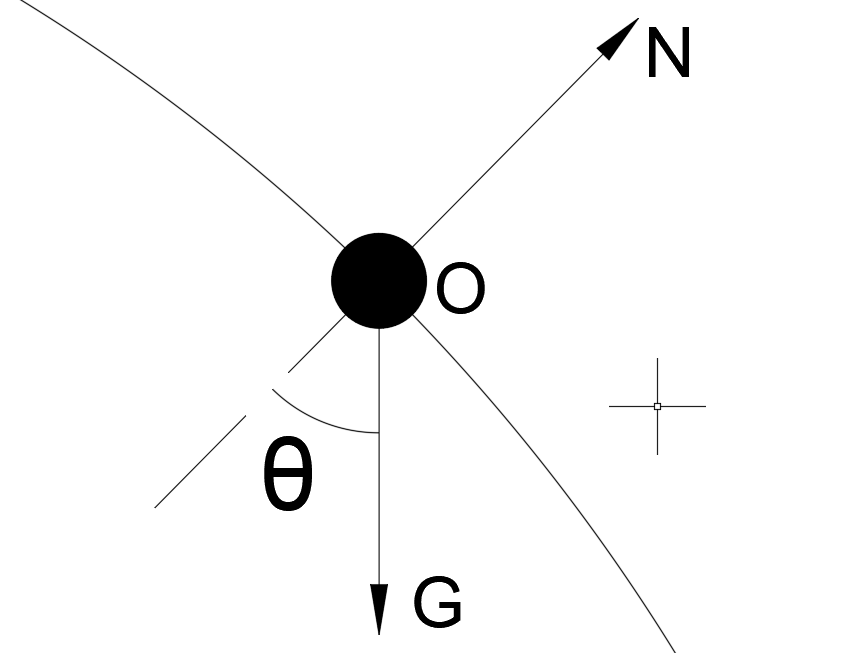
\includegraphics[height=100pt]{Chp2_illus2.png}\\
	图2\\
	\raggedright 由图2,对小球应用牛顿第二定律:
	\[m\frac{v^2}{R}=mg\cos\theta-N\]
	\centering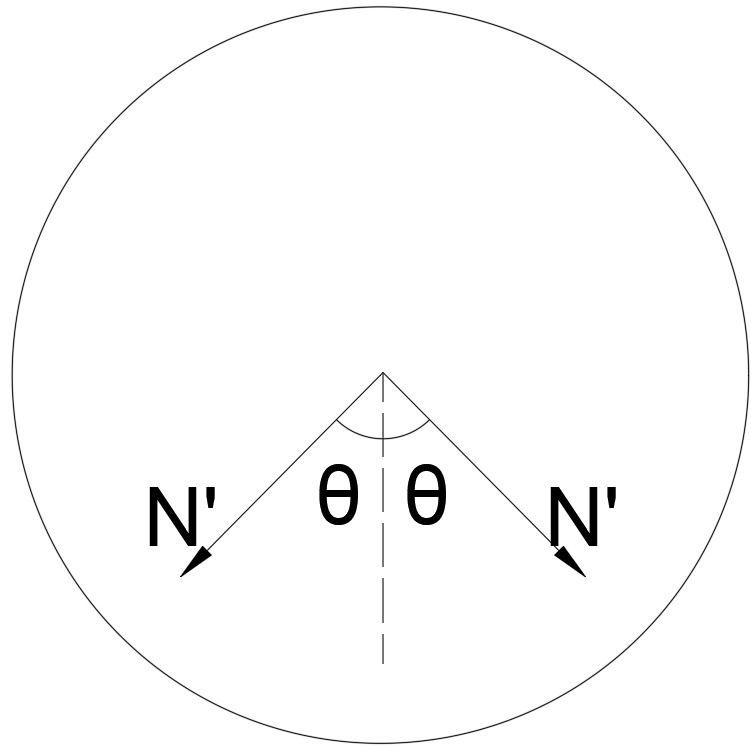
\includegraphics[height=100pt]{Chp2_illus3.png}\\
	图3\\
	\raggedright 由受力分析知,圆环竖直方向受力F为:
	\begin{gather*}
	F=(N'+N')\cos\theta=2N\cos\theta
	\text{当}\theta\in[0,\frac{\pi}{2}]\text{时},\cos\theta>0\\
	\therefore\text{当}N<0\text{时},F\text{向上,圆环上升}\\
	\therefore N=mg\cos\theta-m\frac{v^2}{R}<0\\
	\text{由机械能守恒(见图4):}\frac{1}{2}mv^2=mgh=mg(1-\cos\theta)R\\
	\end{gather*}
	\centering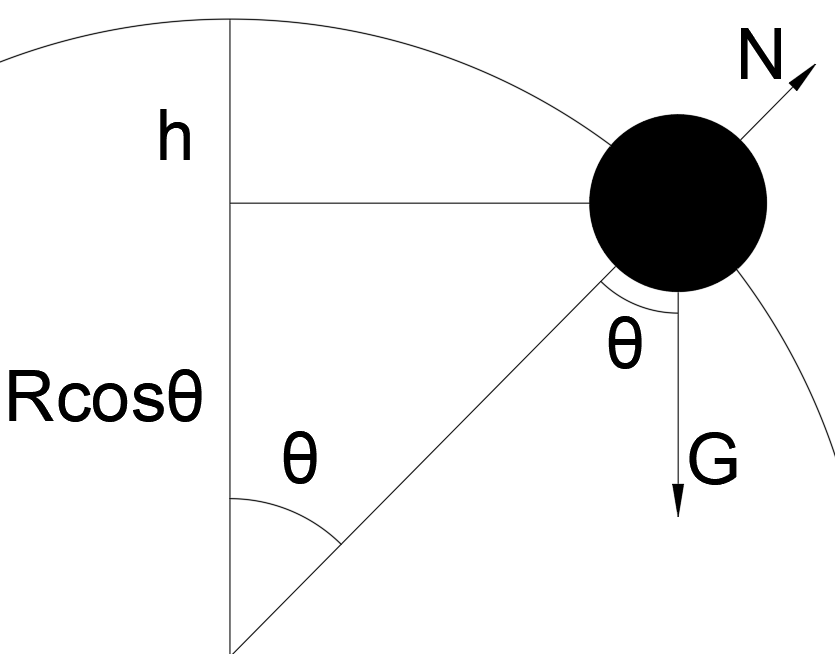
\includegraphics[height=100pt]{Chp2_illus4.png}\\
	图4
	\begin{gather*}
	\text{代入,}\therefore mg\cos\theta-2mg(1-\cos\theta)<0\\
	\therefore 3\cos\theta<2,\quad \theta>\arccos\frac{2}{3}\\
	\text{即当}\theta>\arccos\frac{2}{3}\text{时,圆环会上升}
	\end{gather*}
	\raggedright
	24.
	\begin{gather*}
	T_1\text{提供}G1+G2\\
	\therefore k_1\Delta l=(m_1+m_2)g\\
	\Delta l=\frac{(m_1+m_2)g}{k_1}\\
	\text{由机械能守恒:}\\
	-mgx+\frac{1}{2}k_1(\Delta l+x)^2+\frac{1}{2}m_1v^2=0+\frac{1}{2}k_1(\Delta l)^2+0
	\end{gather*}
	\begin{align*}
	\therefore v&=\sqrt{\frac{-kx^2-2(k_1\Delta l-m_1g)x}{m_1}}\\
	&=\sqrt{-\frac{k_1}{m_1}x^2-\frac{2m_2g}{m_1}x}
	\end{align*}
	利用二次函数最大值为$\frac{4ac-b^2}{4a}$的性质:
	\begin{align*}
	v_{max}	&=\sqrt{\frac{0-\frac{4m_2^2g^2}{m_1^2}}{4\left(-\frac{k_1}{m_1}\right)}}\\
	&=\sqrt{\frac{m_2^2g^2}{m_1k_1}}=\frac{0.3\times 9.8}{\sqrt{0.5\times 8.9\times 10^4}}\\
	&=0.0139(m/s)
	\end{align*}


	
	\section{第三章}
	

		\subsection{选择题}
			1.A
			
			小球受到重力和弹簧弹力做的功,动能不守恒。小球受到的合外力不为0,因此动量不守恒。
			
			2.D
			
			两船在过程中受到了人的摩擦力的作用,合外力不为零,动量不守恒。
			
			3.C
			
			碰撞前后两球动量守恒,因此总动量为0,说明碰撞前两球动量大小相同,方向相反。
			
			4.D
			
			两球碰撞后一起运动,说明为完全非弹性碰撞,存在机械能损失,因此机械能不守恒。两球还受到了弹簧弹力作用,合外力不为零,动量不守恒。
			
			5.D
			
			运动半周前后小球的速度大小不变,方向相反,因此冲量大小\(I=m\Delta v=2mv=2mr \omega\)。
			
			6.C
			
			A人向右跳落入B船后,由动量守恒,A船具有向左的速度,A人具有向右的速度,落入B船后使得A人,B人,B船都具有了向右的速度。B人再跳回A船后,由动量守恒,B人获得的动量朝左,A人和B船获得的动量向右,因此最终B船的速度向右,\(v_B>0\)。B人和A船的动量都向左,因此最终B人落入A船后,A船速度向左,\(v_A<0\)。
			
			7.A
			
			由公式\(E=\frac{p^2}{2m}\),\(p_1=\sqrt{2mE}\),\(p_2=\sqrt{2\times 4m\times E}=2\sqrt{2mE}\)(此处\(p_1\),\(p_2\)均为大小)。由于两个质点面对面运动,\(p_1\)和\(p_2\)符号相反,因此系统动量大小为\(p=p_2-p_1=\sqrt{2mE}\)。
			
			8.A
			
			小球转一周后速度大小和方向都与转前相同,因此动量增量为0,A对。由冲量定义式\(I=F\Delta t\),\(F\)和\(\Delta t\)均不为0,因此\(I\)也不为0,B错,同理可知C错误。在转动过程中小球速度的方向发生了改变,因此过程中动量不守恒,D错。
			
			9.C
			
			小球下落直到与板碰撞之前,对小球分析,有\(v=\sqrt{2gh}\),对板和弹簧分析,设此时弹簧的压缩量为\(x_0\),则由胡克定律有\(x_0=\frac{Mg}{k}\);此后对球与板的碰撞过程,有动量守恒\(mv=(m+M)v_0\),解得,\(v_0=\frac{m}{m+M}\sqrt{2gh}\);此后,小球与板一起运动,设弹簧最大压缩量为\(x\),由能量守恒,\(\frac{1}{2}(m+M)v_0^2+(M+m)gx+\frac{1}{2}kx^2=\frac{1}{2}k(x+x_0)^2\),代入数据解得,\(x=\frac{mg}{k}(1+\sqrt{1+\frac{2kh}{(M+m)g}})\),所以选择C项。
			
			10.A
			
			两球碰撞后以相同速度运动,则为完全非弹性碰撞,必有机械能损失,与完全弹性碰撞矛盾,A错误;若两球碰撞前速度大小相同,方向相反,则碰撞后速度互换,B正确;完全弹性碰撞的定义即为机械能守恒的碰撞,C正确;碰撞过程中动量守恒,D正确。
		\subsection{填空题}
			11. $10m/s$
			
			以人和船为系统,过程中所受外力为$ 0 $,因此动量守恒。有
			\begin{equation*}
			(m+M)v=m(v'+\frac{v}{2})+M\frac{v}{2} 
			\end{equation*}
			代入数据解得$ v'=10m/s $
			
			12. $ m\sqrt{2gh} $ \hspace{4em} 竖直向下
			
			$(1)$由$ I=\Delta p=F\Delta t $,小球下落时间为$\Delta t=\sqrt{\frac{2h}{g}}$,下落过程所受合外力为$F=mg$,故动量增量为
			\begin{equation*}
			\Delta p=mg\cdot\sqrt{\frac{2h}{g}}=m\sqrt{2gh}
			\end{equation*}
			
			$(2)$由合外力(重力)方向竖直向下,可得动量增量方向竖直向下。
			
			13.$\frac{5}{3}N\cdot s$,方向与力的方向同向 \hspace{2em} $\frac{5}{6}N$
			
			由冲量定义,$I = \int F \di t$,对于本题来说,$F$是时间的函数,所以有
			\begin{equation*}
			I = \int_0^1 2t \di t + \int_1^2 2(2-t)^2 \di t = \frac{5}{3}N \cdot s
			\end{equation*}
			平均冲力为
			\begin{equation*}
			\overline{F} = \frac{I}{t} = \frac{5}{6} N
			\end{equation*}
			
			14.$-m\vec{v}$
			
			对全过程,由动量定理,$\vec{I} = \Delta \vec{p} = -m\vec{v}$。
			
			15.$2350kg\cdot m/s$ \hspace{2em} 与跑弹飞行方向相反
			
			由动量定理,$I = \Delta p = m(v-v_0)$,代入数据得$I=2350kg\cdot m/s$,因为炮弹为减速运动,所以冲量方向与炮弹飞行方向相反。
			
			16.$\frac{m+M}{m}\sqrt{2 \mu gs}$
			
			设子弹刚发射时的速度为$v_0$,子弹射入木块后共速速度为$v$。对子弹射入木块的过程,有动量守恒$mv_0=(M+m)v$,此后木块和子弹共同运动,由动能定理
			\begin{equation*}
			\frac{1}{2}(m+M)v^2=\mu (m+M)gs
			\end{equation*}
			代入数据解得
			\begin{equation*}
			v_0=\frac{m+M}{m}\sqrt{2 \mu gs}
			\end{equation*}
			
			17.$\sqrt{\frac{kMl_0^2}{(M+m)^2}}$ \hspace{4em} $\sqrt{\frac{M}{M+nm}}l_0$
			
			分析:每次油滴落入容器等价于油滴与容器发生了一次完全非弹性碰撞,该过程满足动量守恒;此后直到下一滴油滴落入容器之前,整体运动满足能量守恒。
			
			求解:当弹簧第一次达到原长即容器第一次到达滴管下方(第一滴油滴未滴入)时,设容器速度为$v_0$,由能量守恒
			\begin{equation*}
			\frac{1}{2}Mv_0^2=\frac{1}{2}kl_0^2
			\end{equation*}
			可得
			\begin{equation*}
			v_0=\sqrt{\frac{k}{M}}l_0
			\end{equation*}
			再设第$n$滴油滴滴入容器后容器与油滴整体的速度为$v_n$;由动量守恒$P_0=P_n$,其中初状态动量$P_0=Mv_0$,第$n$滴油滴滴入后动量$P_n=(M+nm)v_n$,解得
			\begin{equation*}
			v_n=\frac{M}{M+nm}v_0
			\end{equation*}
			此后容器达到偏离$O$点的最大运动距离$x_n$过程中,由能量守恒,有
			\begin{equation*}
			\frac{1}{2}(M+nm)v_n^2=\frac{1}{2}kx_n^2
			\end{equation*}
			成立,从中可解出
			\begin{equation*}
			x_n=\sqrt{\frac{M+nm}{k}}v_n
			\end{equation*}
			
			故当$n=1$时,
			\begin{equation*}
			v_1=\sqrt{\frac{kMl_0^2}{(M+m)^2}}
			\end{equation*}
			滴入$n$滴油滴后,容器偏离$O$点的最大距离为
			\begin{equation*}
			x_n=\sqrt{\frac{M}{M+nm}}l_0
			\end{equation*}
			
			18.$m(\alpha\sin(\omega t)\vec{i}-(\beta\cos(\omega t)-\beta)\vec{j})$
			
			由已知条件$a_x=\omega\alpha\cos(\omega t),a_y=\omega\beta\sin(\omega t)$,所以$v_x=\int a_x\di t=\alpha\sin(\omega t)+C_1,v_y=\int a_y\di t=-\beta\cos(\omega t)+C_2$,又由初始条件$t=0$时,$vec{v}=0$,可得$C_1=0,C_2=\beta$,所以质点在任一时刻的动量$\vec{p}(t)=m(\alpha\sin(\omega t)\vec{i}-(\beta\cos(\omega t)-\beta)\vec{j})$。
			
			19.$\frac{mv}{\Delta t}$
			
			由平均力计算公式可得$\overline{F}=\frac{I}{\Delta t}=\frac{mv}{\Delta t}$。
			
			20.$\frac{1}{6}m(2v_B-v_A)^2$
			
			因为发生完全弹性碰撞,结合能量守恒,可得碰撞过程中系统动能最小的时刻为弹性势能最大的时刻,亦即A、B共速的时刻,设共速时速度为$v$,则设B运动的方向为正方向由动量守恒有$2mv_B-mv_A=3mv$,此时的动能为
			\begin{equation*}
			E_k=\frac{1}{2}\cdot 3mv^2=\frac{1}{6}m(2v_B-v_A)^2
			\end{equation*}

		\subsection{计算题}
			21.分析:$(1)$动量定理$(2)$因为$\overline{F}>>G$,所以可以忽略重力,再由平均力公式可以求解。
			
			解:$(1)$由动量定理
			\begin{equation*}
			I=\Delta(mv)=m(v_2-v_1)=1.0\times(10+25)=35kg\cdot m/s
			\end{equation*}
			方向竖直向上
			
			$(2)$设球对地面的平均冲力为$F$,地面对球的平均冲力为$F_0$。
			
			对小球撞击地面的过程分析:
			
			因为$\overline{F_0}>>G$,所以可以忽略重力\\
			由平均力计算公式得
			\begin{equation*}
			\overline{F_0}=\frac{I}{t}=\frac{35}{0.02}N=1750N
			\end{equation*}
			再由牛顿第三定律可得
			\begin{equation*}
			\overline{F}=\overline{F_0}=1750N
			\end{equation*}
			方向竖直向下。
			
			22.分析:全过程可分为两部分:一是子弹嵌入木块过程,动量守恒,二是子弹木块整体沿斜面上滑,能量守恒
			
			解:子弹嵌入木块瞬间动量守恒,有
			\begin{equation*}
			mv=(m+M)v`
			\end{equation*}
			再由运动分解,木块速度可分解为垂直于斜面的速度和沿斜面方向的速度,因为木块此后被约束在斜面上运动,所以垂直于斜面的速度突变为$0$,即木块的运动速度为
			\begin{equation*}
			V=v'\cos\theta
			\end{equation*}
			对于木块和子弹的沿斜面上滑过程,有能量守恒
			\begin{equation*}
			\frac{1}{2}(m+M)V^2=(M+m)gl\sin\theta
			\end{equation*}
			联立上述三式可解得:
			\begin{equation*}
			V=\frac{mv\cos\theta}{M+m}
			l=\frac{m^2v^2\cos^2\theta}{2(M+m)^2g\sin\theta}
			\end{equation*}
			
			23.分析:对于碰撞问题可以从能量守恒动量守恒两方面考虑
			
			证明:设运动的小球为球1,质量为$m_1$,静止的小球为球2,质量为$m_2$,碰撞前球1的速度为$\vec{v}_0$,碰撞后球1、球2的速度分别为$\vec{v}_1、\vec{v}_2$,且有$\vec{v}_1$垂直于$\vec{v}_2$。
			
			对碰撞过程:\\能量守恒
			\begin{equation*}
			\frac{1}{2}m_1v_0^2=\frac{1}{2}m_1v_1^2+\frac{1}{2}m_2v_2^2
			\end{equation*}
			即
			\begin{equation}
			v_0^2=v_1^2+\frac{m_2}{m_1}v_2^2
			\end{equation}
			动量守恒
			\begin{equation*}
			m_1\vec{v}_0=m_1\vec{v}_1+m_2\vec{v}_2
			\end{equation*}
			因为$\vec{v}_1$垂直于$\vec{v}_2$
			所以由勾股定理可得
			\begin{equation*}
			m_1^2 v_1^2 + m_2^2 v_2^2 = m_1^2 v_0^2
			\end{equation*}
			\begin{equation}
			v_0^2=v_1^2+\frac{m_2^2}{m_1^2}v_2^2
			\end{equation}
			$(2)-(1)$得
			\begin{equation*}
			\frac{m_2}{m_1}(\frac{m_2}{m_1}-1)v_2^2=0
			\end{equation*}
			因为$v_2^2 \ne 0$且$m_2 \ne 0$,所以
			\begin{equation*}
			\frac{m_2}{m_1}-1=0
			\end{equation*}
			即$m_1=m_2$
			
			得证。
			
			24.分析:将尘埃与飞船共同作为研究对象,则系统动量守恒,从而得到通过$m$与$v$的关系,再通过$\di m$的表达式与前式联立可以消去$\di m$再积分得到$v$和$t$的关系
			
			解:设$t$时刻飞船的质量为$m$,速度为$v$。由初末状态系统动量守恒
			\begin{equation*}
			m_0 v_0=mv
			\end{equation*}
			即
			\begin{equation*}
			m=\frac{m_0 v_0}{v}
			\end{equation*}
			对上式取微分,可得
			\begin{equation}
			\di m=- \frac{m_0 v_0}{v^2} \di v
			\end{equation}
			又有
			\begin{equation}
			\di m=\rho sv\di t
			\end{equation}
			$(3)(4)$联立消去$\di m$再求积分,可得
			\begin{equation*}
			-\int_{v_0}^v \frac{\di v}{v^3}=\int_0^t \frac{\rho s}{m_0 v_0} \di t
			\end{equation*}
			
			解得
			\begin{equation*}
			v=\sqrt{\frac{m_0}{\rho sv_0 t+m_0}v_0}
			\end{equation*}


	\section{第四章}
	\begin{note}
		\noindent 笔者并不建议按照转动定理等名称记忆刚体运动的公式。实际上这些公式都是质点运动学各定律的延伸(如角动量对应动量,转动惯量对应质量,转动定理和动量矩定理对应牛顿第二定律等),做题的时候只需要认定该问题需要用质点运动学的哪些定律,再将质量,力等物理量换成刚体运动学中的转动惯量,力矩等即可。但为了与课本表述一致,在本解析中仍然按照刚体运动学公式名称引用,但会在其后附注数学表达式以方便对应。
	\end{note}
		\subsection{选择题}
			1.C
			
			直观地理解,两个系统所受合外力均为$ Mg $,图A要驱动滑轮和重物(他们都获得了加速度),图B只需要驱动滑轮,因此$ \beta_A<\beta_B $。驱动滑轮的力为$ T_A $和$ T_B $,因此必有$ T_A<T_B $。\par
			从定量计算来看,显然$ T_B=F=Mg $。对A滑轮,对物体应用牛顿第二定律$F=ma$,对滑轮应用转动定律$M=J\beta$:
			\[Mg-T_A=Ma\]
			\[T_A\times R=J\beta\]
			与$ a=\beta R $联立解得:
			\[T_A=\frac{Mg}{\frac{MR^2}{J}+1}\]
			则有$ T_A< Mg=T_B$
			
			2.D
			
			%此处需要配一个图来说明\theta,与竖直方向的夹角,从\pi/2到0
			\begin{tikzpicture}
			\draw[dashed](0,0) -- (3,0);
			\draw[dashed](0,0) -- (0,-3);
			\draw[dashed](3,0) arc (0:-90:3);
			\draw(0,0) -- (2.4,-1.8);
			\draw(0.5,0) arc (0:-36.87:0.5) node[right=5pt] {$ \theta $};
			\end{tikzpicture}\par
			首先此题讨论的是细棒对于$ O $点的转动惯量。由于细棒对于其一个端点的转动惯量恒为$ \frac{1}{3}ml^2 $,因此转动惯量不变。至于角加速度$ \beta $,由转动定律$M=J\beta$:
			\[Mg\frac{l}{2}\sin\theta=\frac{1}{3}ml^2\times\beta\]\par
			解得:$ \beta=\frac{3Mg\sin\theta}{2ml} $,可知$ \beta $随下落过程中$ \theta $的减少而减少,因此角加速度从大到小。
			
			3.D
			
			本题默认水平圆盘放在桌子上,力矩均指对轴的力矩。在玻璃球自由滚动的时候,系统受三个力:重力,支持力(与重力抵消,合力矩为0),还受轴对圆盘的支持力,但由于该力的$ \vec{r}=0 $,因此该力力矩也为0,合外力矩也为0。由动量矩定理$ M=\dy{L}{t} $知,此系统角动量守恒,D正确。若小球处于滚动状态,则轴对圆盘可能会有支持力的作用,由冲量定理$ (I=\Delta p) $,动量不守恒,A,B均错误。若小球与轴或者盘边缘碰撞,由于题目中未说明小球与轴或盘边缘的碰撞是否是完全弹性碰撞,因此碰撞可能会产生机械能损失,C错误。\\
			\begin{note}
			笔者希望同学们对这类圆盘(或细棒)受到固定轴约束转动的问题有更多了解。轴对圆盘的力有且仅有两个,分别是摩擦力和支持力。对于支持力,其垂直于作用面,因此总是指向轴心,$ \vec{r}=0 $,该力对转轴的力矩为0。至于摩擦力,由于其与相对转动速度相反,因此该力与轴相切,由于轴是有半径的(不是一条线),因此$ \vec{r}=R $(R为转轴的半径,显然摩擦力的力矩不为0(但在碰撞过程中,由于$ \Delta t\to 0 $,由动量矩定理,该力矩导致的角动量变化$ \Delta L\to 0 $,因此也可认为角动量守恒)。该题中已经说明忽略轴的摩擦,因此圆盘和小球受到的合外力矩为0。更多相关内容请参考《力学(物理类)》(舒幼生著)。
			\end{note}
			
			4.C
			
			角动量的定义为$ L=\vec{r}\times m\vec{v} $,$ m $为质点质量,$ \vec{v} $为质点速度(运动状态),$ \vec{r} $为质点的向径(与坐标原点有关),C正确,ABD均错误。
			
			5.D
		
			%此处插一张图
			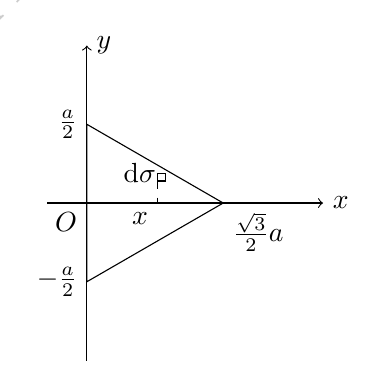
\begin{tikzpicture}
			\zbj{-0.5}{3}{-2}{2}
			\draw (0,-1) node[left] {$ -\frac{a}{2} $}
			-- (0,1) node[left] {$ \frac{a}{2} $}
			-- (1.732,0) node[below right] {$ \frac{\sqrt{3}}{2}a $}
			-- cycle;
			\draw [dashed](0.9,0.28) -- (0.9,0);
			\node[dashed,below left] at (0.9,0) {$ x $};
			\draw (0.9,0.280) rectangle (1,0.38) node [left]{$\di{\sigma}$};
			\end{tikzpicture}\par
			微元$ \di{\sigma} $到轴的距离为$ x $。由于积分域关于$ x $轴对称,被积函数关于$ y $为偶函数,因此$ J=2J_1 $,$ J_1 $为第一象限部分的转动惯量。
			\begin{align*}
			J&=2\iint\limits_{\sigma_1}\left(m\frac{\di{\sigma}}{\frac{\sqrt{3}}{4}a^2}\right)x^2\\
			&=\frac{8m}{\sqrt{3}a^2}\int_0^{\frac{\sqrt{3}}{2}a}\di{x}\int_0^{\frac{1}{2}a-\frac{\sqrt{3}}{3}x}x^2\di{y}
			%&=\frac{8m}{\sqrt{3}a^2}\int_0^{\frac{\sqrt{3}}{2}a}\di{x}\left(\frac{1}{2}ax^2-\frac{\sqrt{3}}{3}x^3\right)\\
			%&=\frac{8m}{\sqrt{3}a^2}\left(\frac{1}{6}ax^3-\frac{\sqrt{3}}{12}x^4\right)\left.\right|_0^{\frac{\sqrt{3}}{2}a}\\
			%&=\frac{8m}{\sqrt{3}a^2}\left(\frac{\sqrt{3}}{16}a^4-\frac{3\sqrt{3}}{64}a^4\right)\\
			%&=\frac{8m}{\sqrt{3}a^2}\frac{\sqrt{3}}{64}a^4\\
			%&=\frac{1}{8}ma^2
			\end{align*}\par
			解得:$ J=\frac{1}{8}ma^2 $
			
			6.A
			
			直观上理解,$ \sigma(\theta) $在$ \theta=\frac{\pi}{2} $时最大,在$ \theta=0 $或$ \theta=\pi $时最小,此即球面质量更多地分布在赤道附近,两极附近质量面密度小。由于赤道附近距离$ z $轴距离更大,因此分布不均匀的球面转动惯量更大,A正确。\par
			通过计算也可以得到相同的结论,此处不再赘述。
			
			7.A
			
			碰撞过程中$ \Delta t\to 0 $,小球和系杆组成的系统受到4个力:重力,支持力(与重力相互抵消),O点对杆的支持力,O点对杆的摩擦力。因此系统角动量守恒(详细分析可见选择题3的“注”部分),有:
			\[0+rmv=(\frac{1}{12}ml^2+m\left(\frac{l}{2}\right))^2\omega\]
			解得:$\omega=\frac{3v}{2l}$
		
			8.C
			
			%此处少一张图
			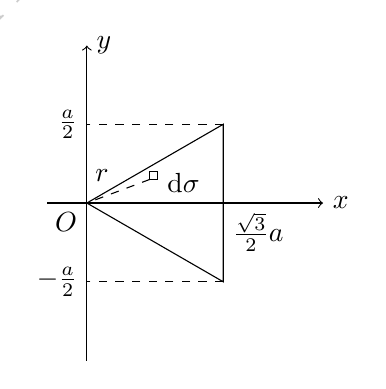
\begin{tikzpicture}
			\zbj{-0.5}{3}{-2}{2}
			\draw (0,0)-- (1.732,1) -- (1.732,-1) -- cycle;
			\draw[dashed] (1.732,1) -- (0,1) node[left] {$ \frac{a}{2} $};
			\draw[dashed] (1.732,-1) -- (0,-1) node[left] {$ -\frac{a}{2} $};
			\node[below right] at (1.732,0) {$\frac{\sqrt{3}}{2}a$};
			\draw (0.8,0.3) rectangle (0.9,0.4);
			\draw [dashed](0.8,0.3) -- node[above left] {$ r $} (0,0);
			\node [below right] at (0.9,0.5) {$\di{\sigma}$};
			\end{tikzpicture}\par
			微元$ \di{\sigma} $到轴(就是到原点)的距离为$ \sqrt{x^2+y^2} $。由于积分域关于$ x $轴对称,被积函数关于$ y $为偶函数,因此$ J=2J_1 $,$ J_1 $为第一象限部分的转动惯量。
			\begin{align*}
			J&=2\iint\limits_{\sigma_1}\left(m\frac{\di{\sigma}}{\frac{\sqrt{3}}{4}a^2}\right)(x^2+y^2)\\
			&=\frac{8m}{\sqrt{3}a^2}\int_0^{\frac{\sqrt{3}}{2}a}\di{x}\int_0^{\frac{\sqrt{3}}{3}x}(x^2+y^2)\di{y}
			\end{align*}\par
			解得:$ J=\frac{5}{12}ma^2 $
			
			9.A
			
			由动量矩定理易知A正确。BCD均为充分条件。小球在绳子的束缚下绕定点做匀速圆周运动,则所受合外力不为0(绳子的拉力),B错误,且小球受到的重力和支持力对定点的力矩均不为0,因此受到了外力矩的作用,C错误。对于D,可令$ J=t,\omega=\frac{1}{t} $,则$ L=J\omega=1 $,角动量守恒,但转动惯量和角速度都在随时间变化,因此D错误。
			
			10.A
			
			卫星做匀速圆周运动,则$ m,v,r $均不变,$ \vec{r}\times\vec{v} $的方向也不变,因此角动量守恒。卫星与地球的万有引力与卫星的运动方向恒垂直,因此卫星与地球构成的系统的内力(万有引力)不做功,同时又不受外力作用,因此卫星的动能守恒。
	\subsection{填空题}
			\[11.\frac{3M}{ma} \hspace{2em} \frac{18M^2}{m^2a^3}t^2\]\par
			本题中转动方向固定,用标量形式计算即可。
			\begin{gather*}
			\beta=\frac{M}{J}=\frac{6M}{ma^2}\\
			\text{开始时}\omega=0,\quad\therefore \omega=\frac{6M}{ma^2}t\\
			v=\omega r=\frac{6M}{ma^2}t\times\frac{a}{2}=\frac{3M}{ma}t\\
			\alpha_{\tau}=\dy{v}{t}=\frac{3M}{ma}\\
			\alpha_n=\frac{v^2}{r}=\frac{\left(\frac{3M}{ma}t\right)^2}{\frac{a}{2}}=\frac{18M^2}{m^2a^3}t^2
			\end{gather*}
			\[12.\frac{1}{12}mR^2\omega_0^2\]\par
			圆柱所受合外力为摩擦力$f$,效果使得圆柱的质心运动速度$ v_c $增大。\par
			圆柱所受合外力矩为摩擦力矩$ M_f $,效果使得圆柱的角速度$ \omega $减小。\par
			圆柱做纯滚动的瞬间,即$ v_c=\omega R $。因此求得$ v_c $和$ \omega $对时间的函数,解出$ t $即可。\par
			对圆柱使用牛顿第二定律$F=ma$和转动定律$M=J\beta$:
			\begin{gather*}
			a_c=\frac{f}{m}=\mu g\quad\therefore v_c=0+\mu gt=\mu gt\\
			\beta=\frac{M}{J}=\frac{-\mu mgR}{\frac{1}{2}mR^2}=-\frac{2\mu g}{R}\\
			\therefore \omega=\omega_0+\beta t=\omega_0-\frac{2\mu g}{R}t\\
			\text{代入纯滚关系式:}\mu gt=\omega_0R-2\mu gt\\
			\therefore t=\frac{\omega_0R}{3\mu g}\\
			\text{此时}v_c=\mu g\frac{\omega_0R}{3\mu g}=\frac{\omega_0R}{3}\\
			\hspace{2em}\omega=\omega_0-\frac{2\mu g}{R}\frac{\omega_0R}{3\mu g}=\frac{\omega_0}{3}
			\end{gather*}\par
			由柯尼希定理:
			\begin{align*}
			E_{\text{总}}&=\frac{1}{2}mv_c^2+\frac{1}{2}J\omega^2\\
			&=\frac{1}{2}m\left(\frac{\omega_0R}{3}\right)^2+\frac{1}{2}\left(\frac{1}{2}mR^2\right)\left(\frac{\omega_0}{3}\right)^2\\
			&=\frac{1}{12}mR^2\omega_0^2
			\end{align*}
			\[14.\frac{1}{8}Mg\]
			物体加速度$ a $与滑轮角加速度$ \beta $的关系为:
			\[\beta=\frac{a}{R}=\frac{g}{4R}\]
			对滑轮应用转动定律$M=J\beta$:
			\begin{gather*}
			TR=\frac{1}{2}MR^2\beta\\
			\therefore T=\frac{MR^2}{2R}\frac{g}{4R}=\frac{1}{8}Mg
			\end{gather*}
			\[15.\frac{1}{2l}\left(\sqrt{\frac{3gl}{2}}+\frac{v_0}{2}\right)\]\par
			首先计算碰撞前杆的角速度,由机械能守恒:
			\begin{gather*}
			0+0=Mg(-\frac{l}{2}\sin 30^\circ)+\frac{1}{2}J\omega^2\\
			\omega_1=\sqrt{\frac{Mgl}{4}\frac{2}{\frac{1}{3}Ml^2}}=\sqrt{\frac{3g}{2l}}
			\end{gather*}\par
			以杆和子弹为系统,在碰撞过程中,所受外力里只有O点对杆的支持力为无穷大(抵消子弹沿杆方向的速度),但该力产生的力矩为0,因此碰撞过程中系统角动量守恒,有:
			\begin{gather*}
			l\sin 30^\circ mv_0+J\omega_1=(J+ml^2)\omega\\
			\therefore \omega=\frac{1}{2l}\left(\sqrt{\frac{3gl}{2}}+\frac{v_0}{2}\right)
			\end{gather*}
			\[16.\frac{1}{4}mR^2 \]\par		
			均匀圆形薄板对圆心的转动惯量$ J=\frac{1}{2}mR^2 $,由垂直轴定理,$ J=J_1+J_2 $,$ J_1,J_2 $分别为薄板对其自身一条直径的转动惯量(两条相互垂直的直径)。由于圆板为圆对称,对任意一条直径的转动惯量相同,因此$ J_1=J_2 $,则$ J_1=\frac{1}{2}J=\frac{1}{4}mR^2 $
			\[17.J_1=J_2\]\par
			记薄板对垂直于自身并穿过中心的轴的转动惯量为$ J $。\par
			由对称性,薄板分别相对于两条对角线的转动惯量相等,分别相对过其中心且平行于一边的轴的转动惯量也相等。\par
			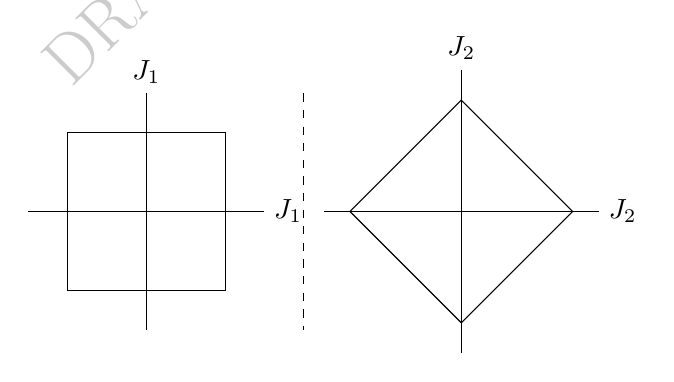
\begin{tikzpicture}
			\draw (-1,-1) rectangle (1,1);
			\draw (1.5,0) node[right] {$ J_1 $} -- (-1.5,0);
			\draw (0,1.5) node[above] {$ J_1 $} -- (0,-1.5);
			\draw [dashed] (2,1.5) -- (2,-1.5);
			\draw [rotate around={45:(4,0)}] (3,-1) rectangle (5,1);
			\draw (5.75,0) node[right] {$ J_2 $} -- (2.25,0);
			\draw (4,1.8) node[above] {$ J_2 $} -- (4,-1.8);
			\end{tikzpicture}\par
			由垂直轴定理,$ J=2J_1=2J_2 $,因此$ J_1=J_2 $。
			\[18.75rad/s\]\par
			物块受到重力,支持力(相互抵消),绳的拉力。由于绳的向径与拉力的方向在同一条直线上,因此小物块所受合外力矩为0,角动量守恒。则:
			\begin{gather*}
			(mR_1^2)\omega_0=(mR_2^2)\omega\\
			\therefore \omega=\frac{R_1^2}{R_2^2}\omega_0=\frac{0.5^2}{0.1^2}\times 3=75(rad/s)
			\end{gather*}
			\[19.0\]\par
			棒球沿直线飞行,则速度$ \vec{v} $的方向沿该直线,向径$ \vec{r} $的方向也沿该直线,因此角动量$ L=\vec{r}\times m\vec{v}=0 $
			\[20.2\sqrt{\frac{g\sin\theta}{3l}}\]\par
			由机械能守恒:
			\begin{gather*}
			\hspace{1pt}2mg\left(\frac{l}{2}\sin\theta\right)+mg\left(-\frac{l}{2}\sin\theta\right)+0+0\\
			=0+0+\frac{1}{2}\left(2m\left(\frac{l}{2}\right)^2\right)\omega^2+\frac{1}{2}\left(m\left(\frac{l}{2}\right)^2\right)\omega^2\\
			\therefore \omega=2\sqrt{\frac{g\sin\theta}{3l}}
			\end{gather*}

		\subsection{计算题}
			\[21.\frac{m}{m+\frac{1}{2}M}\frac{Sg}{rl}\] 
			
			对左端下垂链条应用牛顿第二定律$F=ma$,对上端链条和飞轮应用转动定律$M=J\beta$,右端下垂链条应用牛顿第二定律$F=ma$:
			\begin{gather}
			m\frac{l-\pi r+S}{2l}g-T_1=m\frac{l-\pi r+S}{2l}a\\
			(T_1-T_2)r=\left(\frac{1}{2}Mr^2+m\frac{\pi r}{l}r^2\right)\beta\\
			T_2-m\frac{l-\pi r-S}{2l}g=m\frac{l-\pi r-S}{2l}a\\
			\text{代入}a=\beta r,(1)+\frac{(2)}{r}+(3):\notag
			\end{gather}
			\begin{align*}
			m\frac{S}{l}g&=m\frac{l-\pi r}{l}\beta r+\left(\frac{1}{2}M+\frac{m\pi r}{l}\right)\beta r\\
			&\left(m+\frac{1}{2}M\right)\beta r
			\end{align*}
			\[\therefore \beta=\frac{m}{m+\frac{1}{2}M}\frac{Sg}{rl}\]
			\[22.a=\frac{2}{7}g\]
			$ \because $人相对绳子加速度为0,绳子相对地面加速度为0\\
			$ \therefore $人相对地面加速度为a\\
			对人应用牛顿第二定律$F=ma$,对滑轮应用转动定律$M=J\beta$,对重物应用牛顿第二定律$F=ma$:
			\begin{gather}
			mg-T_1=ma\\
			(T_1-T_2)R=\frac{1}{4}mR^2\alpha\\
			T_2-\frac{1}{2}mg=\frac{1}{2}ma
			\end{gather}
			\[(1)+\frac{(2)}{R}+(3):\]
			\begin{align*}
			\frac{1}{2}mg&=\frac{3}{2}ma+\frac{1}{4}ma\\
			&=\frac{7}{4}ma
			\end{align*}
			\[\therefore a=\frac{2}{7}g\]
			\[23.\Delta x=31.36m,\Delta\theta=78.4rad.(g=9.8m/s^2)\]
			\[\text{或}\Delta x=32m,\Delta\theta=80rad.(g=10m/s^2)\]
			本解析取$ g=9.8m/s^2 $。以物体初始位置为原点,竖直向下为x轴建立坐标系。由能量守恒:
			\begin{align*}
			0+0+0&=mg(-x)+\frac{1}{2}mv^2+\frac{1}{2}\left(\frac{1}{2}MR^2\right)\omega^2\\
			gx&=\frac{1}{2}v^2+\frac{1}{4}\frac{M}{m}v^2\\
			\frac{g}{\frac{1}{2}+\frac{M}{4m}}x&=\left(\dy{x}{t}\right)^2\\
			\sqrt\frac{g}{\frac{1}{2}+\frac{M}{4m}}\di{t}&=\frac{\di{x}}{\sqrt{x}}\\
			\therefore \sqrt\frac{g}{\frac{1}{2}+\frac{M}{4m}}t&=2\sqrt{x}+C
			\end{align*}
			代入$ t=0,x=0,\therefore c=0 $
			\begin{gather*}
			\therefore \frac{gt^2}{2+\frac{M}{m}}=x\\
			\therefore x\left.\right|_{t=4s}=\frac{16g}{2+\frac{15}{5}}=\frac{16}{5}g=31.36(m)\\
			\theta=\frac{x}{R}=\frac{16g}{5\times 0.4}=8g=78.4(rad)
			\end{gather*}
			\[24.\frac{3m_2^2(v_1+v_2)^2}{m_1^2l\mu g}\]\par
			本题所述力矩,全部指对O点的力矩。\par
			撞击前后瞬间,子弹和细棒组成的系统仅受O点支持力,因此合外力矩为0。由角动量守恒:
			\begin{gather*}
			lm_2v_1+0=-lm_2v_2+\frac{1}{3}m_1l^2\omega\\
			\therefore \omega=\frac{3m_2(v_1+v_2)}{m_1l}
			\end{gather*}\par
			摩擦力对O点力矩:
			\begin{align*}
			M	&=\int_{r=0}^{r=l}fr=\int_{r=0}^{r=l}\mu \di{m}gr\\
			&=\int_0^l\mu gr\left(m_1\frac{\di{r}}{l}\right)\\
			%&=\frac{\mu m_1g}{l}\frac{r^2}{2}\left.\right|^l_0\\
			&=\frac{\mu m_1gl}{2}
			\end{align*}
			\begin{align*}
			\text{又}\because M&=J\dy{\omega}{t}\\
			&=J\dy{\omega}{\theta}\dy{\theta}{t}=J\dy{\omega}{\theta}\omega
			\end{align*}
			\begin{gather*}
			\therefore \frac{M}{J}\di{\theta}=\omega\di{\omega}\\
			\text{由}\theta=0\text{时},\omega=0\\
			\therefore \frac{M}{J}\theta=\frac{1}{2}\omega^2
			\end{gather*}
			\begin{align*}
			\therefore \theta&=\frac{\omega^2}{2}\frac{J}{M}\\
			&=\frac{1}{2}\frac{9m_2^2(v_1+v_2)^2}{m_1^2l^2}\frac{\frac{1}{3}m_1l^2}{\frac{\mu m_1gl}{2}}\\
			&=\frac{3m_2^2(v_1+v_2)^2}{m_1^2l\mu g}
			\end{align*}
		\end{multicols}
	
	
\end{document}